% Preamble
\documentclass[12pt, aspectration=1610]{beamer}
\usetheme{Copenhagen}
\usecolortheme{beaver}

\setbeamertemplate{navigation symbols}{}

\usepackage{hyperref}
\usepackage{csquotes}
\usepackage{graphicx}


\usepackage{tikz}
\usetikzlibrary{arrows.meta,
                backgrounds,
                chains,
                positioning,
                shapes.geometric, shapes.multipart
            }

\title{Python dictionaries from scratch}
\author{Kai Striega}
\date{2025-04-03}

\begin{document}

    \maketitle

    \begin{frame}{Who am I?}
        \begin{itemize}
            \item Self taught developer
            \item Senior software engineer at Cartesian Software 
            \item Volunteer in the Free and Open Source community
            \item SheCodes mentor in Python, Linux and git
        \end{itemize}
        \begin{center}
            \includegraphics[scale=0.2]{ images/headshot.jpg}
        \end{center}
    \end{frame}

    \begin{frame}{The Agenda}
        \begin{itemize}
            \item Look at what a dictionary is
            \item Look at how they would normally be implemented
            \item Look at CPython's implementation
        \end{itemize}
    \end{frame}

    \begin{frame}{Why Dictionaries?}
        \begin{itemize}
            \item Play an extremely important role in Python
            \item Used in almost every Python program
            \item The interpreter requires dictionaries to run code
            \item Important to know how the tools that you use everyday work 
        \end{itemize}
    \end{frame}

    \begin{frame}{Introducing the Dictionary}
        \begin{itemize}
            \item The CPython documentation introduces dictionaries as:
            \item ``It is best to think of a dictionary as a set of key: value pairs, with the requirement that the keys are unique (within one dictionary)''
        \end{itemize}
    \end{frame}
    
    \begin{frame}{The interface}
        \begin{itemize}
            \item The interface defines how an object should behave, and what operations can be performed
            \item The interface for dictionaries in CPython is very large, we won't be covering the entire interface
            \item Some common behaviours include:
                \begin{itemize}
                    \item Dictionary creation $d = \text{\{k: v\}}$
                    \item Setting a key value pair $d[k] = v$
                    \item Retrieving a given value $d[k]$ 
                    \item Deleting a given value $\text{del }d[k]$
                \end{itemize}
        \end{itemize}
    \end{frame}

    \begin{frame}{How to implement an interface}
        \begin{itemize}
            \item There are multiple ways to implement the same interface
                \begin{enumerate}
                    \item A hashmap or hash table
                    \item A linked list with linear search to access the elements
                    \item A search tree
                \end{enumerate}
            \item CPython's implementation uses a hashmap - with some interesting twists
        \end{itemize}
    \end{frame}

    \begin{frame}{Hashmaps}
        \begin{itemize}
            \item Map a key to a value using a \textit{hash} function
            \item Very common data structure, available in almost every language
            \item Very interesting data structure, lots of potential optimisation/tricks
            \item Very old data structure, first published in 1953!
        \end{itemize}
    \end{frame}

    \begin{frame}{Hashmap: A visual approach}
        \begin{tikzpicture}[
            node distance = 7mm and 4mm,
              start chain = going right, 
               arr/.style = {semithick, -Stealth},
               dot/.style = {circle, fill, inner sep=1.2pt,
                             label=left:####1},
            every label/.append style = {font=\footnotesize, fill=white, align=center,
                                         fill opacity=0.5, text opacity=1, 
                                         inner sep=1pt},
                 E/.style = {ellipse, draw, fill=####1},
              mpnh/.style = {rectangle split, rectangle split horizontal, 
                             rectangle split parts=3, draw, fill=gray!20,
                             inner sep=2pt,
                             on chain},
              mpnv/.style = {rectangle split, rectangle split parts=10,
                 rectangle split part fill={gray!30,gray!10,gray!30,gray!30,gray!30,
                                            gray!10,gray!30,gray!10,gray!10,gray!30},
                 draw, minimum height=2ex},
               sym/.style = {yshift=-1mm},
               syp/.style = {yshift=+1mm},
                                    ]
            \node[mpnv, label=H] (H) 
                {\nodepart{one}     $\diagup$
                 \nodepart{two}     \vphantom{$\diagup$} 
                 \nodepart{three}   $\diagup$
                 \nodepart{four}    $\diagup$
                 \nodepart{five}    $\diagup$
                 \nodepart{six}     \vphantom{$\diagup$} 
                 \nodepart{seven}   $\diagup$
                 \nodepart{eight}   \vphantom{$\diagup$} 
                 \nodepart{nine}    \vphantom{$\diagup$} 
                 \nodepart{ten}     $\diagup$
                };
            %
            \node[mpnh, right=of H.two east] (A1) 
               {\nodepart{one}  $\diagup$
                \nodepart{two}  $k_1$
                \nodepart{three}    \hphantom{$\diagup$}  
               };
            \node[mpnh] (A2)
               {\nodepart{one}      \hphantom{$\diagup$}
                \nodepart{two}      $k_4$
                \nodepart{three}    $\diagup$
               };
            %
            \node[mpnh, right=of H.six east] (B1)
               {\nodepart{one}      $\diagup$
                \nodepart{two}      $k_5$
                \nodepart{three}    \hphantom{$\diagup$}
               };
            \node[mpnh] (B2)
               {\nodepart{one}      \hphantom{$\diagup$}
                \nodepart{two}      $k_2$
                \nodepart{three}    \hphantom{$\diagup$}
               };
            \node[mpnh] (B3)
               {\nodepart{one}      \hphantom{$\diagup$}
                \nodepart{two}      $k_7$
                \nodepart{three}    $\diagup$ 
               };
            %
            \node[mpnh, right=of H.eight east] (C1)
               {\nodepart{one}      $\diagup$
                \nodepart{two}      $k_3$
                \nodepart{three}    $\diagup$
               };
            %
            \node[mpnh, right=of H.nine east] (D1)
               {\nodepart{one}  $\diagup$
                \nodepart{two}  $k_8$
                \nodepart{three}    \hphantom{$\diagup$}
               };
            \node[mpnh] (D2)
               {\nodepart{one}      \hphantom{$\diagup$}
                \nodepart{two}      $k_6$
                \nodepart{three}    $\diagup$
               };
            %% arrows (right)
            \draw[arr]  (H |- H.two east)   edge (A1)
                        (H |- H.six east)   edge (B1)
                        (H |- H.eight east) edge (C1)
                        (H |- H.nine east)   to (D1)
                        ;
            \draw[arr, transform canvas={yshift=1mm}]  
                        (A1.three north |- A1.east)  edge (A2)
                        (B1.three north |- B1.east)  edge (B2)
                        (B2.three north |- B2.east)  edge (B3)
                        (D1.three north |- D2)   to   (D2)
                        ;
            \draw[arr, transform canvas={yshift=-1mm}]
                        (A2.one north |- A2)  edge  (A1)
                        (B2.one north |- B2)  edge  (B1)
                        (B3.one north |- B3)  edge  (B2)
                        (D2.one north |- D2)   to   (D1)
                        ;
            %% dots, ellipses
            \pgfmathsetseed{3}
            Explicitly sets the seed for
            \foreach \i in {1,2,...,8}
                \node (k\i) [dot=$k_{\i}$] at (-33mm +40*rand,0.5*rand) {};


            \scoped[on background layer]
            {
            \draw[fill=gray!30]  (-4,0.4) ellipse (3 and 2);
            \path   (-4,1) node[label={$U$\\ (universe of keys)}] {};

            \draw[fill=white]   (-4,0) ellipse (2.4 and 1);
            \path   (-6,0) node[label=right:$K$\\ (actual\\ keys)] {};

            \draw[arr]  (k1)    edge ([syp] H.two west)
                        (k4)    edge ([sym] H.two west)

                        (k2)    edge ([syp] H.six west)
                        (k5)    edge (H.six west)
                        (k7)    edge ([sym] H.six west)
                        
                        (k3)    edge (H.eight west)
                        
                        (k8)    edge ([syp] H.nine west)
                        (k6)    edge ([sym] H.nine west)
                        ;
                }
        \end{tikzpicture}
    \end{frame}
    \begin{frame}{How CPython implements dictionaries}
        \begin{itemize}
            \item CPython does it differently
            \item CPython defines three files that define the dictionary data structure
                \begin{itemize}
                    \item \href{https://github.com/python/cpython/blob/3.12/Include/dictobject.h}{dictobject.h} defines the C interface
                    \item \href{https://github.com/python/cpython/blob/3.12/Objects/dictobject.c}{dictobject.c} implements the C interface 
                    \item \href{https://github.com/python/cpython/blob/3.12/Objects/dictnotes.txt}{dictnotes.txt} describes why design decisions were made
                \end{itemize}
        \end{itemize}
    \end{frame}

    \begin{frame}{And first, there was data}
        \begin{itemize}
            \item To store \textit{any} data we must first have somewhere to store it
            \item Hashmaps usually do this via an underlying data structure called an Array
            \item Arrays are contiguous and homogeneous blocks of memory
        \end{itemize}
    \end{frame}

    \begin{frame}{What we have so far}
        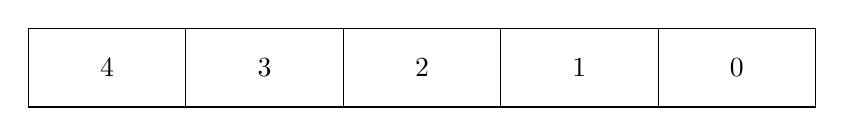
\begin{tikzpicture}
            \node[draw, minimum width=2cm, minimum height=1cm] at (8, 0) {0};
            \node[draw, minimum width=2cm, minimum height=1cm] at (6, 0) {1};
            \node[draw, minimum width=2cm, minimum height=1cm] at (4, 0) {2};
            \node[draw, minimum width=2cm, minimum height=1cm] at (2, 0) {3};
            \node[draw, minimum width=2cm, minimum height=1cm] at (0, 0) {4};
        \end{tikzpicture}
    \end{frame}
    \begin{frame}{Accessing the Array}
        \begin{itemize}
            \item We can access the array using indices, or offsets, from the start of the array
            \item However we want to be able to convert any Python object $O$ to an index
            \item For this we will use a special function $H$ to \textit{hash} $O$
            \item More generally, a \textit{hash function} is any function that takes a variable sized input into a fixed size output
        \end{itemize}
    \end{frame}
    \begin{frame}{Exploring Python's hash function}
        \begin{itemize}
            \item Luckily for us, Python provides a hash function ``hash''
            \item We can see how hash works by a couple of examples
                \begin{itemize}
                    \item $\textit{hash}(``PythonWA'') = -4886646145239673352$ 
                    \item $\textit{hash}(15) = 15$ - Note: Integers always hash to themselves!
                    \item $\textit{hash}(("PythonWA", 15)) = -8383856720255659210$ 
                \end{itemize}
        \end{itemize}
    \end{frame}

    \begin{frame}{What makes a hash function ``good''? }
        A list of (some) properties of a good hash function:
        \begin{itemize}
            \item Fast: who likes waiting? 
            \item Deterministic: We want to be able to retrieve the key again 
            \item Uniform: This reduces the chance of \textit{collisions} where two keys generate the same index
        \end{itemize}
    \end{frame}
 
    \begin{frame}{Fitting hashes into our array}
        \begin{itemize}
            \item $-4886646145239673352$ will not fit into our array 
            \item To convert the hash to indices we can take the remainder of the size of the array 
            \item e.g. $-4886646145239673352 \mod 5 = 3$
        \end{itemize}

        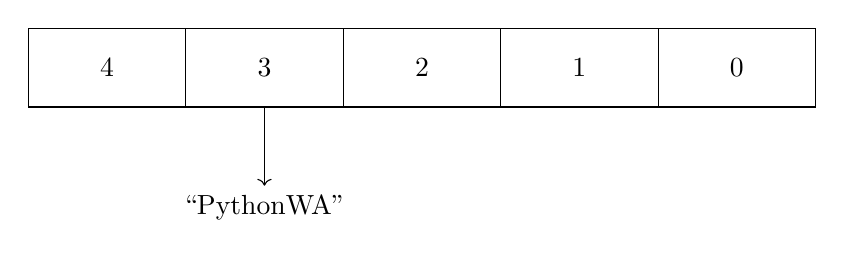
\begin{tikzpicture}
            \node[draw, minimum width=2cm, minimum height=1cm] at (8, 0) {0};
            \node[draw, minimum width=2cm, minimum height=1cm] at (6, 0) {1};
            \node[draw, minimum width=2cm, minimum height=1cm] at (4, 0) {2};
            \node[draw, minimum width=2cm, minimum height=1cm] at (2, 0) {3};
            \node[draw, minimum width=2cm, minimum height=1cm] at (0, 0) {4};
            \draw[->] (2, -0.5) -- (2, -1.5) node[below] {``PythonWA''};
        \end{tikzpicture}
    \end{frame}

    \begin{frame}{Hash Collisions}
        \begin{itemize}
            \item Let's use two numbers as our keys, 12 and 17
            \item Integers hash to themselves, so $\text{hash}(12) = 12$
            \item Now 12 is inserted at $12 \mod 5 = 2$
        \end{itemize}
        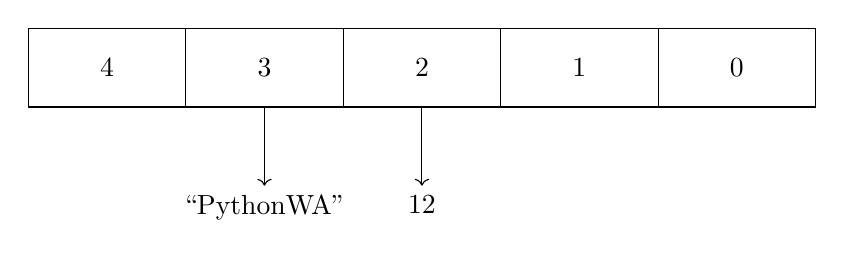
\begin{tikzpicture}
            \node[draw, minimum width=2cm, minimum height=1cm] at (8, 0) {0};
            \node[draw, minimum width=2cm, minimum height=1cm] at (6, 0) {1};
            \node[draw, minimum width=2cm, minimum height=1cm] at (4, 0) {2};
            \node[draw, minimum width=2cm, minimum height=1cm] at (2, 0) {3};
            \node[draw, minimum width=2cm, minimum height=1cm] at (0, 0) {4};
            \draw[->] (2, -0.5) -- (2, -1.5) node[below] {``PythonWA''};
            \draw[->] (4, -0.5) -- (4, -1.5) node[below] {12};
        \end{tikzpicture}
    \end{frame}
 
    \begin{frame}{What about 17?}
        \begin{itemize}
            \item The hash of 17 is itself (as 17 is an integer)
            \item It will also be inserted at $17 \mod 5 = 2$
            \item There are \textit{many} solutions for dealing with this. But there are two broad categories:
                \begin{enumerate}
                    \item Separate Chaining
                    \item Open Addressing
                \end{enumerate}
        \end{itemize}
    \end{frame}
    \begin{frame}{Separate Chaining}
        \begin{itemize}
            \item Big Idea: Combine the elements in each bucket in some data structure and search it
            \item Canonically the data structure is a linked list 
        \end{itemize}
        \begin{tikzpicture}
            \node[draw, minimum width=2cm, minimum height=1cm] at (8, 0) {0};
            \node[draw, minimum width=2cm, minimum height=1cm] at (6, 0) {1};
            \node[draw, minimum width=2cm, minimum height=1cm] at (4, 0) {2};
            \node[draw, minimum width=2cm, minimum height=1cm] at (2, 0) {3};
            \node[draw, minimum width=2cm, minimum height=1cm] at (0, 0) {4};
            \draw[->] (2, -0.5) -- (2, -1.5) node[below] {``PythonWA''};
            \draw[->] (4, -0.5) -- (4, -1.5) node[below] {12};
            \draw[->] (4, -2.0) -- (4, -2.5) node[below] {17};
        \end{tikzpicture}
    \end{frame}

    \begin{frame}{Open Addressing}
        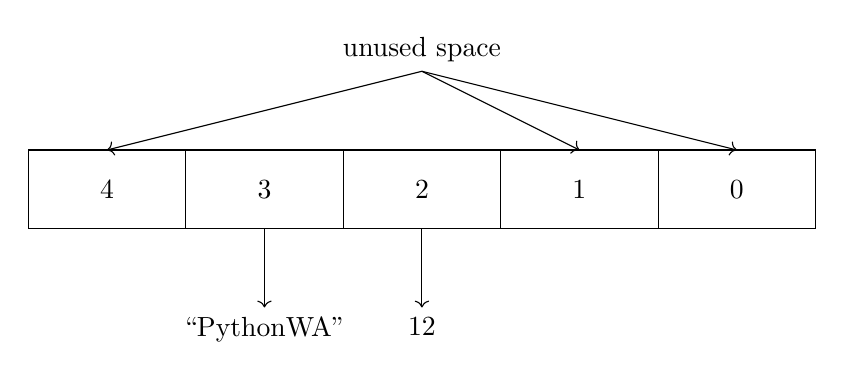
\begin{tikzpicture}
            \node[draw, minimum width=2cm, minimum height=1cm] at (8, 0) {0};
            \node[draw, minimum width=2cm, minimum height=1cm] at (6, 0) {1};
            \node[draw, minimum width=2cm, minimum height=1cm] at (4, 0) {2};
            \node[draw, minimum width=2cm, minimum height=1cm] at (2, 0) {3};
            \node[draw, minimum width=2cm, minimum height=1cm] at (0, 0) {4};
            \draw[<-] (0, 0.5) -- (4, 1.5) node[above] {unused space};
            \draw[->] (2, -0.5) -- (2, -1.5) node[below] {``PythonWA''};
            \draw[->] (4, -0.5) -- (4, -1.5) node[below] {12};
            \draw[<-] (6, 0.5) -- (4, 1.5) node[above] {};
            \draw[<-] (8, 0.5) -- (4, 1.5) node[above] {};
        \end{tikzpicture}
        \begin{itemize}
            \item Big Idea: Utilise the space we have available to store data
            \item 2 of the 5 slots are utilised - why not use them?
            \item The process of finding the next bucket is called \textit{probing}
        \end{itemize}
    \end{frame}
    \begin{frame}{Probing}
        \begin{itemize}
            \item \textit{Linear Probing} looks using the next available slot e.g. $H(O)+1, H(O)+2, H(O)+3, \ldots$ 
            \item \textit{Quadratic Probing} looks using an arbitrary quadratic polynomial e.g. $H(O)+1^2,H(O)+2^2, H(O)+3^2 \ldots$
            \item \textit{Double Hashing} looks using a second hash function e.g. $H(i, O) = (H_1(O) + i H_2(O))$
        \end{itemize}
    \end{frame}

    \begin{frame}{The pros and cons of Linear Probing}
        \begin{itemize} 
            \item As CPython uses a variation of linear probing, I'm going to focus on that a bit
            \item Pros \\
            \begin{itemize}
                \item Simplicity
                \item Locality of reference 
                \item No extra memory requirements
            \end{itemize}
            \item Cons \\
            \begin{itemize}
                \item Primary Clustering
                \item Expensive Deletions
            \end{itemize}
        \end{itemize}
    \end{frame}

    \begin{frame}{Insertions with Open Addressing}
        \begin{itemize}
            \item Many articles claim hashtables pick the next empty bucket, this is a simplification 
            \item For linear probing we use a \textit{linear function} to pick the next bucket
            \item CPython uses a LCG to generate the next number (more on this later) 
        \end{itemize}
    \end{frame}
    
    \begin{frame}{Insertions with Open Addressing}
        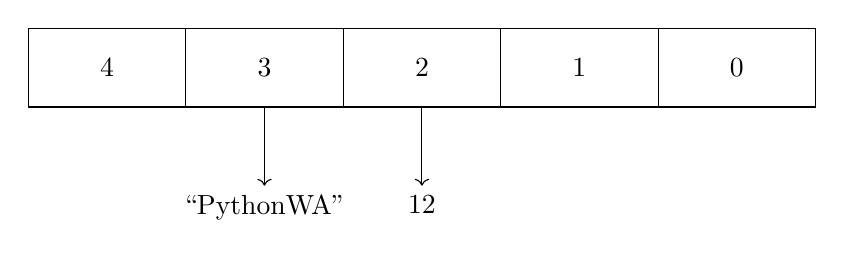
\begin{tikzpicture}
            \node[draw, minimum width=2cm, minimum height=1cm] at (8, 0) {0};
            \node[draw, minimum width=2cm, minimum height=1cm] at (6, 0) {1};
            \node[draw, minimum width=2cm, minimum height=1cm] at (4, 0) {2};
            \node[draw, minimum width=2cm, minimum height=1cm] at (2, 0) {3};
            \node[draw, minimum width=2cm, minimum height=1cm] at (0, 0) {4};
            \draw[->] (2, -0.5) -- (2, -1.5) node[below] {``PythonWA''};
            \draw[->] (4, -0.5) -- (4, -1.5) node[below] {12};
        \end{tikzpicture}
    \end{frame}
    
    \begin{frame}{Insertions with Open Addressing}
        \begin{tikzpicture}
            \node[draw, minimum width=2cm, minimum height=1cm] at (8, 0) {0};
            \node[draw, minimum width=2cm, minimum height=1cm] at (6, 0) {1};
            \node[draw, minimum width=2cm, minimum height=1cm] at (4, 0) {2};
            \node[draw, minimum width=2cm, minimum height=1cm] at (2, 0) {3};
            \node[draw, minimum width=2cm, minimum height=1cm] at (0, 0) {4};
            \draw[->] (2, -0.5) -- (2, -1.5) node[below] {``PythonWA''};
            \draw[->] (4, -0.5) -- (4, -1.5) node[below] {12};
            \draw[->] (4, 0.5) to [out=150, in=30] (2, 0.5); 
        \end{tikzpicture}
    \end{frame}

    \begin{frame}{Insertions with Open Addressing}
        \begin{tikzpicture}
            \node[draw, minimum width=2cm, minimum height=1cm] at (8, 0) {0};
            \node[draw, minimum width=2cm, minimum height=1cm] at (6, 0) {1};
            \node[draw, minimum width=2cm, minimum height=1cm] at (4, 0) {2};
            \node[draw, minimum width=2cm, minimum height=1cm] at (2, 0) {3};
            \node[draw, minimum width=2cm, minimum height=1cm] at (0, 0) {4};
            \draw[->] (2, -0.5) -- (2, -1.5) node[below] {``PythonWA''};
            \draw[->] (4, -0.5) -- (4, -1.5) node[below] {12};
            \draw[->] (2, 0.5) to [out=150, in=30] (0, 0.5); 
        \end{tikzpicture}
    \end{frame}

    \begin{frame}{Insertions with Open Addressing}
        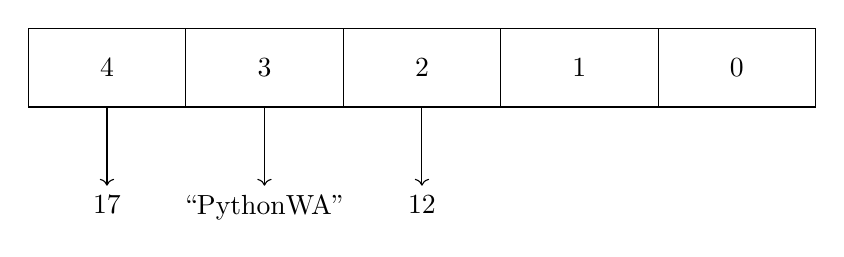
\begin{tikzpicture}
            \node[draw, minimum width=2cm, minimum height=1cm] at (8, 0) {0};
            \node[draw, minimum width=2cm, minimum height=1cm] at (6, 0) {1};
            \node[draw, minimum width=2cm, minimum height=1cm] at (4, 0) {2};
            \node[draw, minimum width=2cm, minimum height=1cm] at (2, 0) {3};
            \node[draw, minimum width=2cm, minimum height=1cm] at (0, 0) {4};
            \draw[->] (2, -0.5) -- (2, -1.5) node[below] {``PythonWA''};
            \draw[->] (4, -0.5) -- (4, -1.5) node[below] {12};
            \draw[->] (0, -0.5) -- (0, -1.5) node[below] {17};
        \end{tikzpicture}
    \end{frame}

    \begin{frame}{Deletions with Linear Probing}
        \begin{itemize}
            \item Deleting buckets is more complicated than adding buckets
            \item If a bucket in the "chain" is removed it cannot find the next bucket
            \item The hashmap will them erroneously tell us the item doesn't exist 
            \item Let's go through an example by trying to delete $17$
        \end{itemize}
    \end{frame}

    \begin{frame}{Deletions with Linear Probing}
        \begin{itemize}
            \item Recall that $12$ and $17$ have the same initial index 
            \item We can't simply delete the bucket there
            \item We have to check whether the key there actually equals the key provided
        \end{itemize}
    \end{frame}

    \begin{frame}{Deletions with Linear Probing}
        \begin{tikzpicture}
            \node[draw, minimum width=2cm, minimum height=1cm] at (8, 0) {0};
            \node[draw, minimum width=2cm, minimum height=1cm] at (6, 0) {1};
            \node[draw, minimum width=2cm, minimum height=1cm] at (4, 0) {2};
            \node[draw, minimum width=2cm, minimum height=1cm] at (2, 0) {3};
            \node[draw, minimum width=2cm, minimum height=1cm] at (0, 0) {4};
            \draw[->] (2, -0.5) -- (2, -1.5) node[below] {``PythonWA''};
            \draw[->] (4, -0.5) -- (4, -1.5) node[below] {12};
            \draw[->] (0, -0.5) -- (0, -1.5) node[below] {17};
            \draw[->] (4, 0.5) to [out=150, in=30] (2, 0.5); 
        \end{tikzpicture}
    \end{frame}

    \begin{frame}{Deletions with Linear Probing}
        \begin{tikzpicture}
            \node[draw, minimum width=2cm, minimum height=1cm] at (8, 0) {0};
            \node[draw, minimum width=2cm, minimum height=1cm] at (6, 0) {1};
            \node[draw, minimum width=2cm, minimum height=1cm] at (4, 0) {2};
            \node[draw, minimum width=2cm, minimum height=1cm] at (2, 0) {3};
            \node[draw, minimum width=2cm, minimum height=1cm] at (0, 0) {4};
            \draw[->] (2, -0.5) -- (2, -1.5) node[below] {``PythonWA''};
            \draw[->] (4, -0.5) -- (4, -1.5) node[below] {12};
            \draw[->] (0, -0.5) -- (0, -1.5) node[below] {17};
            \draw[->] (2, 0.5) to [out=150, in=30] (0, 0.5); 
        \end{tikzpicture}
    \end{frame}

    \begin{frame}{Deletions with Linear Probing}
        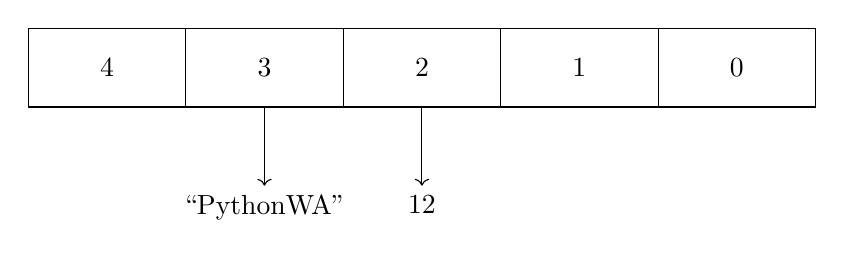
\begin{tikzpicture}
            \node[draw, minimum width=2cm, minimum height=1cm] at (8, 0) {0};
            \node[draw, minimum width=2cm, minimum height=1cm] at (6, 0) {1};
            \node[draw, minimum width=2cm, minimum height=1cm] at (4, 0) {2};
            \node[draw, minimum width=2cm, minimum height=1cm] at (2, 0) {3};
            \node[draw, minimum width=2cm, minimum height=1cm] at (0, 0) {4};
            \draw[->] (2, -0.5) -- (2, -1.5) node[below] {``PythonWA''};
            \draw[->] (4, -0.5) -- (4, -1.5) node[below] {12};
        \end{tikzpicture}
    \end{frame}

    \begin{frame}{What if we try to delete 12?}
        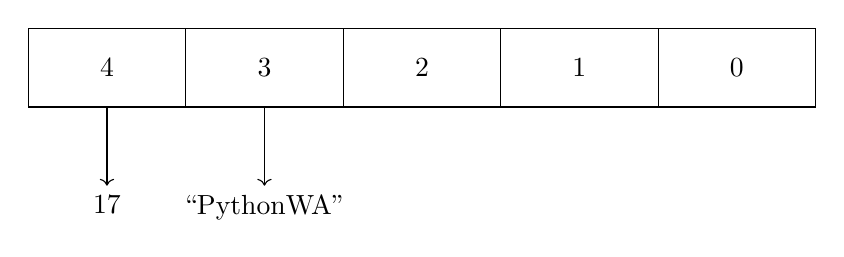
\begin{tikzpicture}
            \node[draw, minimum width=2cm, minimum height=1cm] at (8, 0) {0};
            \node[draw, minimum width=2cm, minimum height=1cm] at (6, 0) {1};
            \node[draw, minimum width=2cm, minimum height=1cm] at (4, 0) {2};
            \node[draw, minimum width=2cm, minimum height=1cm] at (2, 0) {3};
            \node[draw, minimum width=2cm, minimum height=1cm] at (0, 0) {4};
            \draw[->] (2, -0.5) -- (2, -1.5) node[below] {``PythonWA''};
            \draw[->] (0, -0.5) -- (0, -1.5) node[below] {17};
        \end{tikzpicture}
    \end{frame}

    \begin{frame}{\ldots and now access 17?}
        \begin{itemize}
            \item We look for 17 at $H(17) \mod 5 = 2$
            \item However that bucket is empty \ldots
            \item \ldots and so we stop
        \end{itemize}
        \begin{tikzpicture}
            \node[draw, minimum width=2cm, minimum height=1cm] at (8, 0) {0};
            \node[draw, minimum width=2cm, minimum height=1cm] at (6, 0) {1};
            \node[draw, minimum width=2cm, minimum height=1cm] at (4, 0) {2};
            \node[draw, minimum width=2cm, minimum height=1cm] at (2, 0) {3};
            \node[draw, minimum width=2cm, minimum height=1cm] at (0, 0) {4};
            \draw[->] (2, -0.5) -- (2, -1.5) node[below] {``PythonWA''};
            \draw[->] (0, -0.5) -- (0, -1.5) node[below] {17};
            \draw[<-] (4, 0.5) -- (4, 1.5) node[above] {Is $17$ here?};
        \end{tikzpicture}
    \end{frame}

    \begin{frame}{Deleting buckets with probes}
        \begin{itemize}
            \item Naively deleting items causes problems with the \textit{probing sequence}
            \item Two solutions shifting all elements in the sequence and marking the bucket as deleted
            \item Shifting all elements is usually not recommended as it is quite expensive
            \item Marking buckets as deleted defers the work to a time where it is convenient
        \end{itemize}
    \end{frame}

    \begin{frame}{}
        \begin{center}
            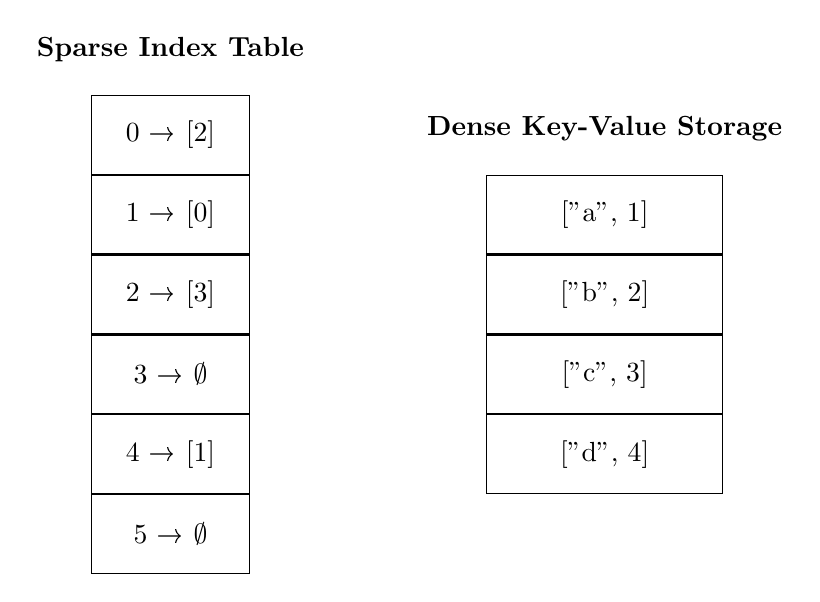
\begin{tikzpicture}
                % Sparse Index Table
                \node (index0) [draw, minimum width=2cm, minimum height=1cm] {0 → [2]};
                \node (index1) [draw, minimum width=2cm, minimum height=1cm, below=0pt of index0] {1 → [0]};
                \node (index2) [draw, minimum width=2cm, minimum height=1cm, below=0pt of index1] {2 → [3]};
                \node (index3) [draw, minimum width=2cm, minimum height=1cm, below=0pt of index2] {3 → $\emptyset$};
                \node (index4) [draw, minimum width=2cm, minimum height=1cm, below=0pt of index3] {4 → [1]};
                \node (index5) [draw, minimum width=2cm, minimum height=1cm, below=0pt of index4] {5 → $\emptyset$};

                % Label for index table
                \node [above=0.3cm of index0] {\textbf{Sparse Index Table}};

                % Key-Value Storage (Dense)
                \node (kv0) [draw, minimum width=3cm, minimum height=1cm, right=3cm of index1] {["a", 1]};
                \node (kv1) [draw, minimum width=3cm, minimum height=1cm, below=0pt of kv0] {["b", 2]};
                \node (kv2) [draw, minimum width=3cm, minimum height=1cm, below=0pt of kv1] {["c", 3]};
                \node (kv3) [draw, minimum width=3cm, minimum height=1cm, below=0pt of kv2] {["d", 4]};

                % Label for key-value storage
                \node [above=0.3cm of kv0] {\textbf{Dense Key-Value Storage}};
            \end{tikzpicture}
        \end{center}
    \end{frame}

    \begin{frame}{}
        \begin{itemize}
            \item 
            \item 
            \item 
            \item 
        \end{itemize}
    \end{frame}
    \begin{frame}{}
        \begin{itemize}
            \item 
            \item 
            \item 
            \item 
        \end{itemize}
    \end{frame}
    \begin{frame}{}
        \begin{itemize}
            \item 
            \item 
            \item 
            \item 
        \end{itemize}
    \end{frame}
    \begin{frame}{}
        \begin{itemize}
            \item 
            \item 
            \item 
            \item 
        \end{itemize}
    \end{frame}
    \begin{frame}{}
        \begin{itemize}
            \item 
            \item 
            \item 
            \item 
        \end{itemize}
    \end{frame}
   
\end{document}
